% ============================================================
% LLM-BLM 小型株のデータ：母集団、生存者バイアス、決算発表文と株価の取得
% コンパイル：tectonic -X compile LLM-BLM_小型株のデータ.tex   （XeTeX 系。このフォルダで実行する）
% 図と数値は 図/（作成スクリプト/figs.py が data/smallcap.sqlite と smallcap/bias.py から作る）
% ============================================================
\documentclass[xelatex,ja=standard,jafont=haranoaji,a4paper,10pt,openany]{bxjsreport}
\setpagelayout*{left=24mm,right=24mm,top=24mm,bottom=26mm,footskip=11mm}

\usepackage{amsmath,amssymb,mathtools,bm}
\usepackage{booktabs,array,multirow,longtable}
\usepackage{graphicx}
\usepackage{adjustbox}
\usepackage{xcolor}
\usepackage{tikz}
\usetikzlibrary{arrows.meta,positioning,calc,fit}
\usepackage{enumitem}
\usepackage{caption}
\usepackage{float}
\usepackage[most]{tcolorbox}
\usepackage[hidelinks,bookmarksnumbered]{hyperref}

\graphicspath{{図/}}

\definecolor{c1}{HTML}{2A78D6}
\definecolor{c2}{HTML}{EB6834}
\definecolor{c3}{HTML}{1BAF7A}
\definecolor{c4}{HTML}{EDA100}
\definecolor{c7}{HTML}{6250D6}
\definecolor{ink2}{HTML}{52514E}
\definecolor{soft1}{HTML}{E4EEF9}
\definecolor{soft2}{HTML}{FBEEDF}
\definecolor{soft3}{HTML}{E3F3E9}
\definecolor{soft4}{HTML}{EEE8FA}
\definecolor{soft5}{HTML}{FDF3DA}

\newcommand{\code}[1]{\texttt{#1}}
\newcommand{\SP}{S\&P500}
\newcommand{\figref}[1]{図~\ref{#1}}
\newcommand{\tabref}[1]{表~\ref{#1}}
\newcommand{\chapref}[1]{第~\ref{#1}~章}

\setlist[itemize]{leftmargin=1.6em,itemsep=0.2em,topsep=0.4em}
\setlist[enumerate]{leftmargin=1.8em,itemsep=0.2em,topsep=0.4em}
\captionsetup{font=small,labelfont=bf,skip=6pt}
\renewcommand{\arraystretch}{1.2}
\setlength{\LTpre}{6pt}
\setlength{\LTpost}{6pt}

\makeatletter
\def\@makechapterhead#1{\vspace*{0.3\Cvs}{\parindent\z@\raggedright\normalfont
  \ifnum\c@secnumdepth>\m@ne\if@mainmatter{\Large\headfont\@chapapp\thechapter\@chappos}\par\nobreak\vskip0.4\Cvs\fi\fi
  \interlinepenalty\@M\LARGE\headfont #1\par\nobreak\vskip 1.5\Cvs}}
\def\@makeschapterhead#1{\vspace*{0.3\Cvs}{\parindent\z@\raggedright\normalfont
  \interlinepenalty\@M\LARGE\headfont #1\par\nobreak\vskip 1.5\Cvs}}
\makeatother

\newtcolorbox{keybox}[1][要点]{enhanced,breakable,colback=soft1,colframe=c1,boxrule=0.5pt,arc=2pt,
  left=8pt,right=8pt,top=6pt,bottom=6pt,title={#1},fonttitle=\sffamily\bfseries\small,coltitle=white}
\newtcolorbox{notebox}[1][注意]{enhanced,breakable,colback=soft2,colframe=c2,boxrule=0.5pt,arc=2pt,
  left=8pt,right=8pt,top=6pt,bottom=6pt,title={#1},fonttitle=\sffamily\bfseries\small,coltitle=white}

\title{LLM-BLM 小型株のデータ\\[6pt]
  \large 母集団の作り方、生存者バイアスの見積もり、\\決算発表文と株価の取得}
\author{データの報告書}
\date{2026 年 10 月 23 日}

\begin{document}
\maketitle

% ============================================================
\chapter*{概要}
\addcontentsline{toc}{chapter}{概要}

\SP{} では、LLM の決算発表文の読み取りは発表の当日に株価に入りきり、翌日以降には残っていなかった（実験 2・8）。追加した参考文献（Hong・Stein 1999、Akbas ほか 2017、Lan ほか）によれば、株価の反応の遅れは注目されていない銘柄に集中する。そこで、\textbf{注目の低い小型株}で同じことを確かめるためのデータを作った。この報告書は、データの作り方と、その偏りの見積もりだけを扱う。\textbf{株価の反応と点数の関係は、まだ一度も計算していない}（事前登録の前）。

\begin{keybox}[要点]
\begin{itemize}
\item \textbf{母集団}：SEC の XBRL から、2015〜2025 年の各年について、米国の提出企業の浮動株時価総額を取り、各年の 1,001〜3,000 位を小型株とした（浮動株時価総額でおおむね 9,000 万〜40 億ドル。Russell 2000 に近い）。後で消えた会社も含めて、一度でも入った会社は 4,921 社。
\item \textbf{生存者バイアス}：無料で取れる株価（yfinance）は、いま上場している会社だけ。小型株の会社・年のうち \textbf{32\%} は株価が取れない（2015 年は 52\%、2025 年は 6\%）。
\item \textbf{消えた理由}：消えた 1,826 社のうち \textbf{79\% が買収}、15\% が倒産。買収された会社は、消える前の 1 年の動きが残った会社とほぼ同じ（浮動株時価総額の中央値 +2\% と +4\%）。倒産した会社は $-22\%$ と、すでに大きく下がっていた。
\item \textbf{集めたデータ}：条件を満たす 2,400 社から 1,000 社を無作為に選び、2015〜2026 年の決算発表文（8-K の EX-99.1）\textbf{38,390 本}（99.0\% が取れた）と、株価、株式数を取った。
\item \textbf{次}：株価の反応を使わない点数付け（辞書、FinBERT、ChronoGPT の埋め込み）を、この PC の GPU で始めた。反応を使う分析は、事前登録の後に行う。
\end{itemize}
\end{keybox}

\tableofcontents

% ============================================================
\chapter{目的}\label{ch:purpose}

\section{これまでの結果}

\begin{itemize}
\item 実験 2〜5・11：LLM の決算発表文の点数は、発表をはさむ 2 取引日の株価の反応を強く説明した（gpt-4o-mini で 1 標準偏差あたり +120bp、先読みのない ChronoGPT でも +34bp）。
\item 実験 2・3・8：その後のドリフト（2〜21 日）と翌日には、有意な残りがなかった。月次・日次の BLM は時価総額加重を上回らなかった（実験 7〜9）。
\end{itemize}

\section{なぜ小型株か}

\begin{longtable}{p{4.4cm}p{9.8cm}}
\toprule
\textbf{文献} & \textbf{この研究への含み} \\
\midrule
\endhead
\bottomrule
\endfoot
Hong・Stein（1999, Journal of Finance） & 情報が投資家の間にゆっくり広がると、短期では反応が足りず（モメンタム）、長期では行き過ぎて戻る。広がりの遅い銘柄ほど、反応の遅れが大きい（理論） \\
Akbas・Markov・Subasi・Weisbrod（2017, SSRN 2860521） & アナリスト予想の処理が遅れるほど、発表時の反応は小さく、その後のドリフトは大きい。非効率は注目されていない銘柄に集中する \\
Lan・Xie・Mi・Zhang（SSRN 4589824） & 投資家の注目が、発表後のドリフトを強める（中国市場、査読前のプレプリント） \\
\end{longtable}

\SP{} は世界で最も注目されている銘柄である。小型株は、アナリストも投資家の注目も少ない。LLM が人の代わりに文章を読む価値は、小型株のほうが大きいはずである。

% ============================================================
\chapter{母集団の作り方}\label{ch:population}

\section{浮動株時価総額で並べる}

Russell 2000 は、米国の上場株を時価総額で並べた 1,001〜3,000 位である。その過去の構成銘柄は無料では手に入らない。そこで、SEC に提出された財務諸表の表紙に載る\textbf{浮動株時価総額}（\code{dei:EntityPublicFloat}）を使って、同じ考え方の範囲を自分で作った。

\begin{itemize}
\item SEC の XBRL の frames（1 回の呼び出しで、全提出企業のある時点の値が取れる API）から、2015〜2025 年の各年の値を取った。浮動株時価総額は決算期の第 2 四半期の末に測るので、年ごとに 4 つの四半期を合わせ、会社・年ごとに 1 つにした。
\item 使わない値：100 万ドル未満（9,406 件。休眠会社など）、4 兆ドル超（100 件。桁を誤った報告）、その会社のほかの年の中央値から 200 倍以上ずれる値（389 件）。
\item 所在地が米国の会社だけを並べ、各年の 1,001〜3,000 位を「小型株の範囲」とした。
\end{itemize}

この作り方では、\textbf{後で上場をやめた会社も、その年の母集団に入る}。SEC の提出は、上場をやめるまで続くからである。

\begin{table}[H]
\centering
\caption{各年の範囲の境目（浮動株時価総額、百万ドル）。}
\label{tab:band}
\small
\setlength{\tabcolsep}{4pt}
\begin{tabular}{lrrrrrrrrrrr}
\toprule
年 & 2015 & 2016 & 2017 & 2018 & 2019 & 2020 & 2021 & 2022 & 2023 & 2024 & 2025 \\
\midrule
米国の提出企業 & 4,846 & 4,619 & 4,520 & 4,483 & 4,338 & 4,470 & 5,114 & 5,024 & 4,629 & 4,416 & 4,283 \\
1,000 位 & 2,552 & 2,269 & 2,637 & 2,907 & 2,800 & 2,559 & 4,100 & 3,200 & 3,368 & 3,623 & 3,935 \\
3,000 位 & 124 & 87 & 99 & 117 & 91 & 106 & 275 & 186 & 115 & 99 & 98 \\
\bottomrule
\end{tabular}
\end{table}

\section{その時点で知られていたか}

浮動株時価総額は、測った日（第 2 四半期の末）の数か月後に、年次報告書（10-K）で公表される。12 月決算の会社なら、6 月末に測り、翌年 3 月までに公表する。そこで、\textbf{測った日の 9 か月後から使える}とする。各判断日の範囲は、そのときに使える最新の値で決める。

% ============================================================
\chapter{生存者バイアス}\label{ch:bias}

\section{どれだけ欠けるか}

無料の株価（yfinance）は、いま上場している会社のものしかない。上場廃止の会社の株価を持つ EODHD は、無料プランでは直近 1 年しか返さない（2026-10-23 に確認）。そこで、\textbf{いま株価が取れる会社だけ}でデータを作り、欠ける分の大きさを見積もった。

範囲に入った会社・年のうち、その年か翌年に決算の 8-K（Item 2.02）を出した 20,282 件を対象にした。いまのティッカーで、その期間の株価が取れるものを「残った」、取れないものを「消えた」とした。

\begin{figure}[H]
\centering
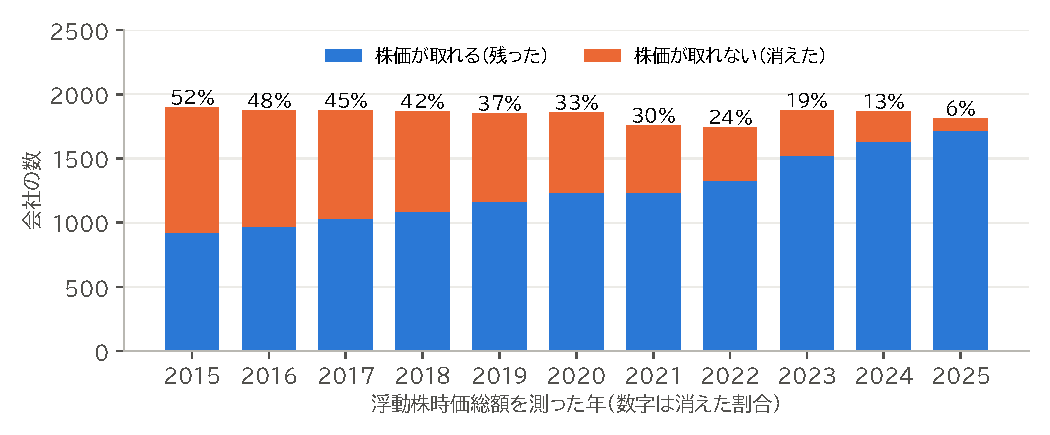
\includegraphics[width=0.92\linewidth]{coverage.pdf}
\caption{小型株の範囲に入った会社（決算の 8-K を出したもの）のうち、株価が取れる会社と取れない会社。}
\label{fig:coverage}
\end{figure}

全体で \textbf{31.7\%}（6,431 件）が欠ける（\figref{fig:coverage}）。古い年ほど多く、2015 年は 51.5\%、2020 年は 33.4\%、2025 年は 5.5\% である。2015 年の小型株は、半分がもう株価を取れない。

\section{なぜ消えたか}

消えた 1,826 社について、EDGAR の届け出から理由を機械的に決めた（上から順に当てはめる）。

\begin{itemize}
\item 倒産：8-K の Item 1.03（倒産・管財人）
\item 買収：合併の委任状（DEFM14A など）、公開買付けへの意見表明（SC 14D9）、8-K の Item 5.01（支配権の移動）
\item 上場廃止・登録廃止：Form 25、Form 15
\item まだ提出している：2026 年にも提出がある（別の市場、名前の変更）
\end{itemize}

\begin{figure}[H]
\centering
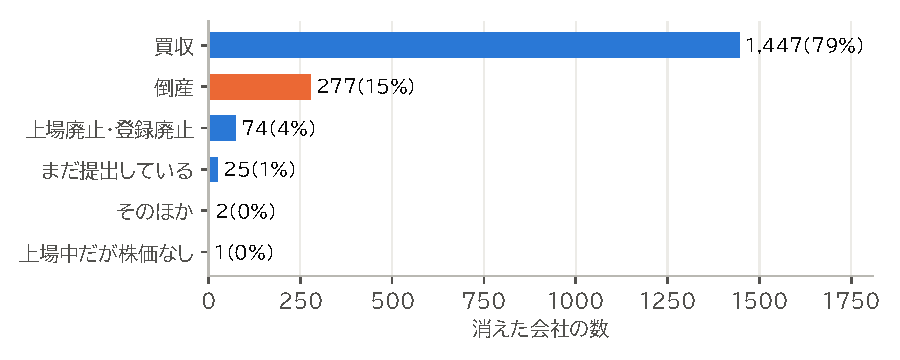
\includegraphics[width=0.78\linewidth]{reasons.pdf}
\caption{消えた会社の理由。}
\label{fig:reasons}
\end{figure}

小型株が消える主な理由は\textbf{買収}（79\%）で、倒産は 15\% だった（\figref{fig:reasons}）。小型株には地方銀行や医薬品・バイオの会社が多く、どちらも合併や買収の多い業種である。

\section{消える前の動き}

消えた会社の株価は取れないので、代わりに、範囲に入った最後の年の、前の年からの浮動株時価総額の変化を見た（株価に株式の数を掛けたものなので、株価の動きの目安になる。ただし株式の発行でも増える）。

\begin{figure}[H]
\centering
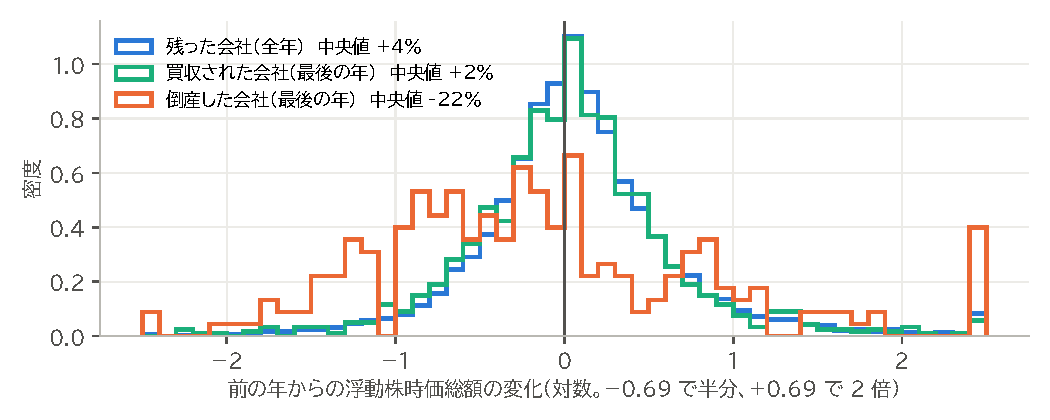
\includegraphics[width=0.92\linewidth]{float_change.pdf}
\caption{前の年からの浮動株時価総額の変化。}
\label{fig:float}
\end{figure}

\begin{table}[H]
\centering
\caption{前の年からの浮動株時価総額の変化。}
\label{tab:float}
\small
\begin{tabular}{lrrr}
\toprule
 & 件数 & 中央値 & 4 割以上減った割合 \\
\midrule
残った会社（全年） & 12,030 & $+4.1\%$ & 11.5\% \\
買収された会社（最後の年） & 1,205 & $+2.3\%$ & 13.9\% \\
倒産した会社（最後の年） & 226 & $\mathbf{-22.0\%}$ & \textbf{38.5\%} \\
上場廃止・登録廃止（最後の年） & 61 & $+9.4\%$ & 13.1\% \\
\bottomrule
\end{tabular}
\end{table}

\section{偏りの向き}

LLM の点数を使う戦略は、「点数の高い会社を多く、点数の低い会社を少なく持つ」形になる。比べる相手は、同じ会社の集合で作った時価総額加重である。

\begin{enumerate}
\item \textbf{倒産（15\%）は、こちらに不利な向き。}倒産した会社は消える前から大きく下がっていた。悪い内容の発表をした会社が抜けるので、点数の低い会社の成績が実際より良く見え、戦略と時価総額加重の差は実際より\textbf{小さく}出る。勝てた場合には、その結果は控えめな見積もりになる。
\item \textbf{買収（79\%）は、向きが読めない。}買収されるときには上乗せで株価が上がるが、その上昇もデータから消える。点数の高い会社と低い会社のどちらが買収されやすいかで、向きが変わる。買収された会社は、消える前の動きが残った会社とほぼ同じだった（\tabref{tab:float}）。
\item \textbf{欠けの多い年は、別の市場を見ている。}2015〜2018 年は半分前後が欠ける。結論は「生き残った小型株の中で」と書く必要がある。
\end{enumerate}

\begin{notebox}[実験のときに決めておくこと]
\begin{itemize}
\item 欠けの少ない 2021 年以降だけの結果も、主な結果と並べて報告する。
\item 時価総額加重は、同じ会社の集合で作る。実際に買える Russell 2000 の ETF（IWM）は生存者バイアスがないので、参考として並べるだけにする。
\item 買収で消えた会社が、点数でどちらに偏るかは、消えた会社の決算発表文も読めば確かめられる（反応は見ない）。今回は株価の取れる会社だけを集めたので、次の段階の候補とする。
\end{itemize}
\end{notebox}

% ============================================================
\chapter{集めたデータ}\label{ch:data}

\section{会社の選び方}

次の条件をすべて満たす 2,400 社から、1,000 社を無作為に選んだ（乱数の種 0）。

\begin{itemize}
\item 2015〜2025 年のどこかで、小型株の範囲に入った。
\item いま Nasdaq・NYSE・NYSE American に上場していて、yfinance で株価が取れる。
\item 2016 年以降に、決算の 8-K（Item 2.02）を 4 本以上出している。
\end{itemize}

選んだ会社の業種は、医薬品（80 社）、州法銀行（54 社）、バイオ（45 社）、ソフトウェア（43 社）、REIT（42 社）が多い。各年に小型株の範囲に入っている社数は、2015 年の 387 社から 2025 年の 718 社まで（\figref{fig:sample}）。古い年ほど少ないのは、前の章の欠けのためである。

\begin{figure}[H]
\centering
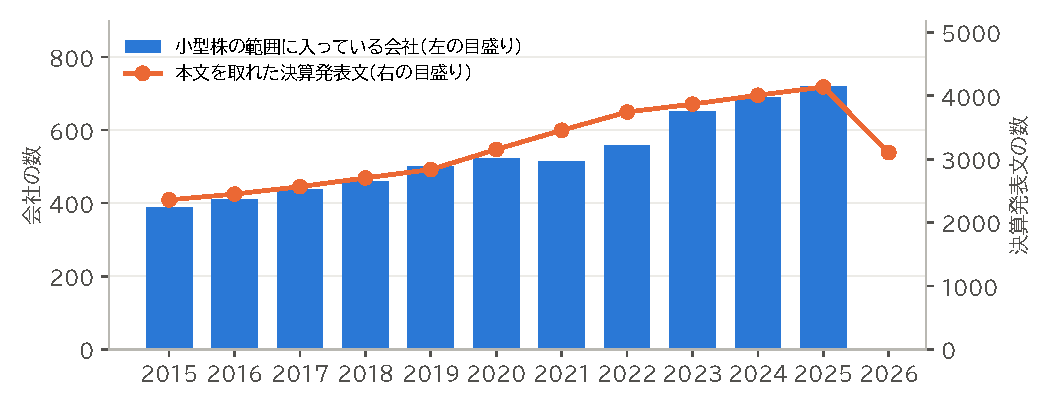
\includegraphics[width=0.92\linewidth]{sample.pdf}
\caption{選んだ 1,000 社のうち、各年に小型株の範囲に入っている会社の数と、本文を取れた決算発表文の数。}
\label{fig:sample}
\end{figure}

\section{決算発表文}

\SP{} と同じ取り方（実験 2 の \code{events/edgar.py}）で、8-K の Item 2.02 に付く EX-99.1 の本文を取った。取得は約 3 時間（SEC の求めに従い、毎秒 8 回以下）。

\begin{table}[H]
\centering
\caption{決算発表文の取得（2015-01-01〜2026-09-30 に提出されたもの）。}
\label{tab:releases}
\small
\begin{tabular}{lr}
\toprule
決算の 8-K（Item 2.02） & 38,800 本（999 社） \\
届け出を読めた & 38,794 本（6 本は SEC の索引が読めなかった） \\
本文を取れた & \textbf{38,390 本}（99.0\%） \\
\quad うち、先頭に EX-99.1（または EX-99）と書かれていた & 99.6\% \\
本文の長さ（中央値） & 24,129 字 \\
反応の日（day 0）が決まった & 99.99\% \\
本文が 4 本以上ある会社 & 998 社 \\
\bottomrule
\end{tabular}
\end{table}

\begin{itemize}
\item 本文の選び方：ファイル名が EX-99.1 に当たるもの 29,991 本、最も大きい添付書類 6,202 本、EX-99.2 などから EX-99.1 に差し替えたもの 723 本。1,305 本は、\SP{} の取得のときにすでに保存していた本文だった（\SP{} に入っていた時期のある会社）。添付書類がなかった届け出は 404 本。
\item 年ごとの本数は、2015 年の 2,358 本から 2025 年の 4,140 本まで増える（2026 年は 9 月までで 3,105 本）。古い年ほど少ないのは、選んだ会社の中で、その年に上場していた会社が少ないためである。
\end{itemize}

\begin{table}[H]
\centering
\caption{届け出が受理された時間帯（ニューヨーク時間）。\SP{} は実験 2 の設計のときの 6,209 本。}
\label{tab:session}
\small
\begin{tabular}{lrr}
\toprule
時間帯 & 小型株 & \SP{} \\
\midrule
寄り前（9:30 より前） & 14.7\% & 23.4\% \\
場中（9:30〜16:00） & 21.4\% & 31.0\% \\
引け後（16:00〜17:30） & 22.3\% & 19.7\% \\
17:30 以後 & \textbf{41.5\%} & 25.9\% \\
\bottomrule
\end{tabular}
\end{table}

小型株は、17:30 より後に受理される届け出が多い（\tabref{tab:session}）。発表文の配信より 8-K の提出が遅れると、反応の日が 1 日ずれうる。\SP{} と同じく、反応の窓を 2 取引日にとって吸収する。

\section{株価と株式数}

\begin{itemize}
\item 株価：範囲に一度でも入り、いま上場している 2,617 社と、指数・ETF（\^{}GSPC、IWM、IJR、SPY、セクター ETF 11 本）。2,632 銘柄のうち 2,627 銘柄が取れた。2014-12 から 2026-09 まで。
\item 発行済株式数：XBRL の frames の \code{dei:EntityCommonStockSharesOutstanding}（四半期ごと、211,112 件）。時価総額は、株式の分割を合わせてから計算する（ポートフォリオを組む段階で行う）。
\end{itemize}

\section{置き場所}

すべて \code{data/smallcap.sqlite}（本体の DB と同じ表の形と、\code{sc\_} で始まる表）。本体の DB は変えていない。本文は \code{data/cache/edgar/}、どちらも Git には入れない。

% ============================================================
\chapter{次にすること}\label{ch:next}

\section{点数付け（実行中）}

株価の反応を使わない点数付けを、この PC の GPU で始めた（\code{smallcap/score.py}）。

\begin{itemize}
\item 辞書（Loughran--McDonald）と、学習なしの FinBERT：\SP{} と同じ設定。
\item ChronoGPT（版 2015）の埋め込み：元の文章の最後の層の平均（実験 5 のベクトル）と、掃除した文章の 3 種類（最後の層の平均、最後のトークン、26 層目の平均）。26 層目は、実験 11 の探索で強かったもの。
\end{itemize}

gpt-4o-mini は、方針どおり最後の比較まで使わない。

\section{事前登録で決めること}

\begin{enumerate}
\item 主な問い：小型株で、LLM（ChronoGPT）の点数は、発表後 2〜60 日の超過リターンを説明するか（2 日の反応を統制したうえで）。
\item 各判断日の小型株の範囲（使える最新の浮動株時価総額で決める）。
\item 超過リターンの基準（IWM、またはセクター ETF）。
\item 統制：数値の驚き、発表前のリターン、規模、モメンタム、業種と四半期。
\item ポートフォリオ：月次の BLM と、同じ会社の集合の時価総額加重。費用は片道 0.3〜0.5\%（小型株の売買の値段の差は大きい）。
\item 欠けの少ない 2021 年以降だけの結果も並べる。
\end{enumerate}

% ============================================================
\chapter{限界}\label{ch:limits}

\begin{itemize}
\item 生き残った会社だけのデータである（\chapref{ch:bias}）。
\item 消えた理由は届け出の種類から機械的に決めた。合併の委任状を出したが成立しなかった会社や、倒産から立ち直った会社の扱いは粗い。
\item 浮動株時価総額の変化は株価の動きの代わりで、株式の発行（バイオ企業に多い）でも増える。
\item 浮動株時価総額は、創業者などの持ち分を除いた値で、Russell 2000 の時価総額とは違う。並べる相手も、上場していない提出企業を含む。
\item 小型株の中でも、選んだ 1,000 社は 2,400 社の一部である。
\end{itemize}

% ============================================================
\chapter*{再現の手順}
\addcontentsline{toc}{chapter}{再現の手順}

\begin{verbatim}
python -m smallcap.build population
python -m smallcap.build submissions
python -m smallcap.build shares
python -m smallcap.build prices
python -m smallcap.bias
python -m smallcap.build select --n 1000
python -m smallcap.build releases
python 資料集/02_実験/小型株のデータ/作成スクリプト/figs.py
powershell -ExecutionPolicy Bypass -File smallcap\start_score.ps1
\end{verbatim}

SEC の手順には \code{SEC\_USER\_AGENT}（名前と連絡先。\code{.env} に置き、表示しない）が要る。設計は \code{設計\_小型株.md}、偏りの数値は \code{smallcap/results/bias.json} と \code{findings.md}、この報告書の数値は \code{図/numbers.json}。

\end{document}
